\documentclass[aspectratio=169]{beamer}
\usepackage[]{multirow}
\usepackage[]{array}
\usepackage[]{graphicx}
\usepackage[T1]{fontenc}
\usepackage[]{url}


\usetheme{default}
\usecolortheme{dove}
\setbeamertemplate{navigation symbols}{}
\setbeamersize{text margin left=.75in, text margin right=.75in}

\title{Demo: Raspberry Pi-Based\\Guitar Environmental Monitor}
\author{Sama Squad (Grant Alphenaar)}
\institute{CIS 641 -- GVSU}
\date{\today}

\begin{document}

  \newcommand{\sectitle}{}

  \begin{frame}
      \titlepage
  \end{frame}
  \begin{frame}{Roadmap}
    \tableofcontents
  \end{frame}

  % Introduction slide
  \renewcommand{\sectitle}{Recap \&c.}
  \section{\sectitle}


    \begin{frame}{\sectitle}{Project Overview}

          Build a system that can\dots
          \begin{itemize}
            \item \dots be run off a Raspberry Pi to\dots
            \item \dots measure temperature and humidity for guitars and\dots
            \item \dots allow user monitoring and (some) control\dots
            \item \dots through a basic web dashboard.
          \end{itemize}

    \end{frame}

    % \begin{frame}{\sectitle}{What?}
    %   \begin{center}
    %     % 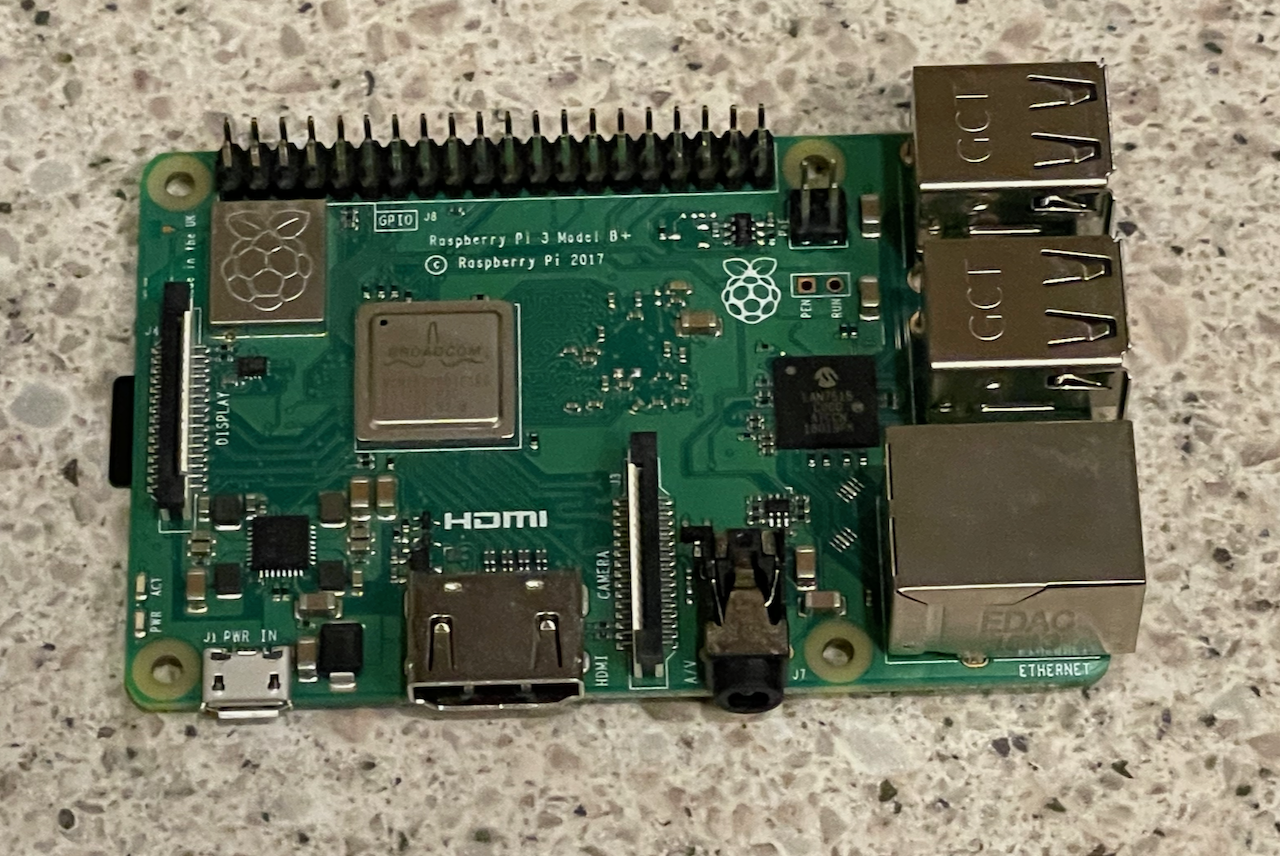
\includegraphics[scale=.20]{images/rpi.png}
    %   \end{center}
    % \end{frame}


  % \renewcommand{\sectitle}{A Bit More Detail\dots}
  % \section{\sectitle}
  % \begin{frame}{\sectitle}{Why?}
  %   \begin{itemize}\LARGE
  %     \item Guitars are (mostly) made out of wood, and\dots
  %     \item \dots wood is sensitive to temperature and humidity\dots
  %     \item \dots especially swings to either extreme\dots
  %     \item \dots which Michigan has a lot of.
  %   \end{itemize}
  % \end{frame}

  % \begin{frame}{\sectitle}{Components}
  %   \begin{columns}
  %     \begin{column}{.5\textwidth}
  %       \centering Sensor Unit:
  %       \vspace*{1em}
  %       \begin{center}
  %         % 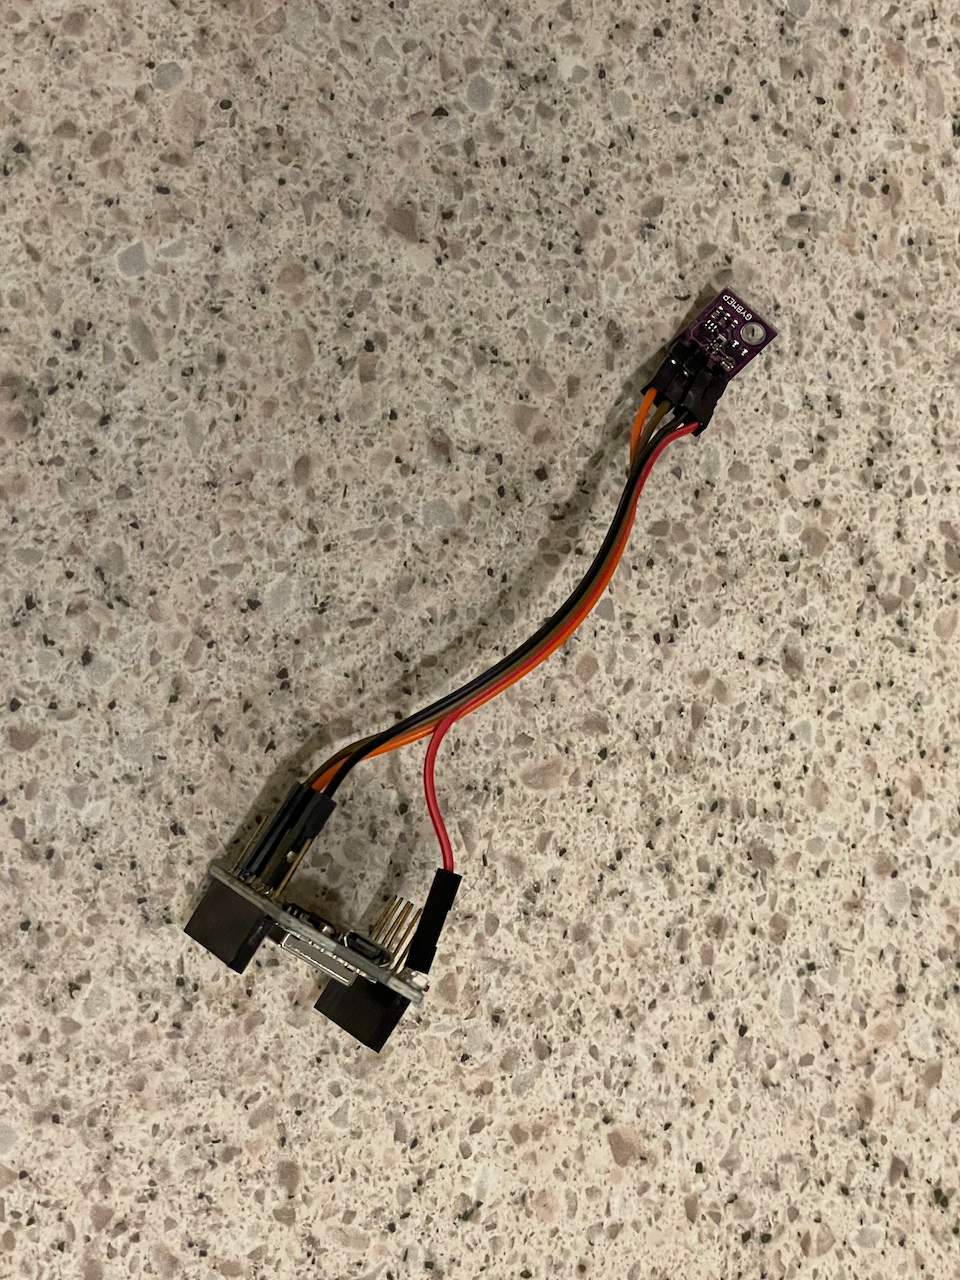
\includegraphics[scale=.1]{images/bme.png}
  %       \end{center}
  %     \end{column}
  %     \begin{column}{.5\textwidth}
  %       \centering Battery Board:
  %       \vspace*{1em}
  %       \begin{center}
  %         % 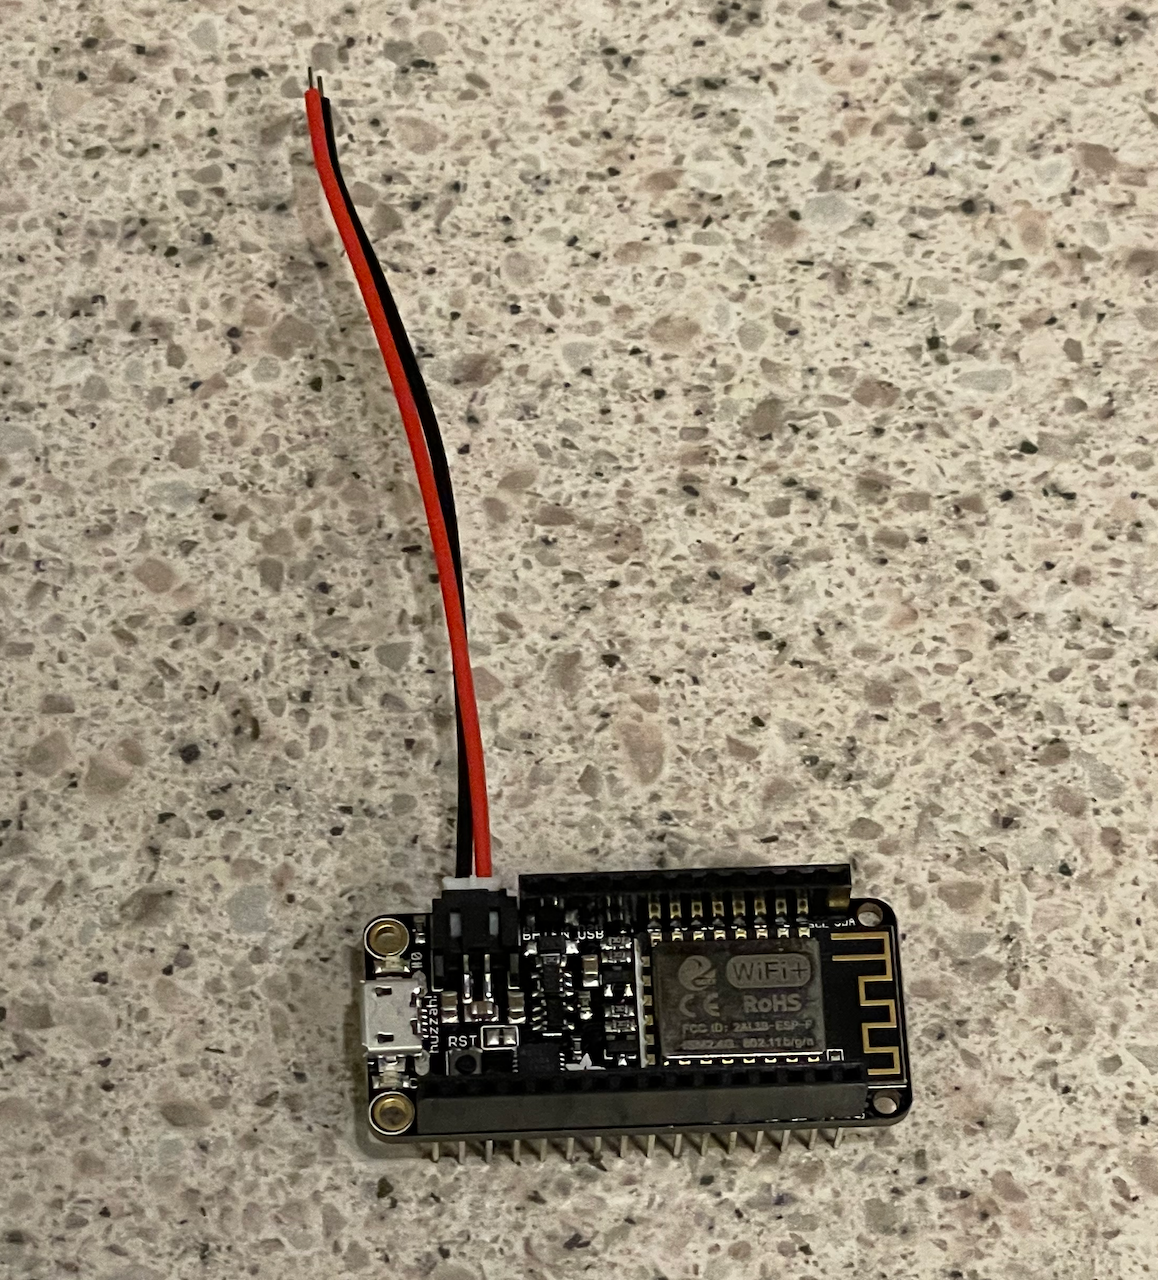
\includegraphics[scale=.1]{images/battery.png}
  %       \end{center}
  %     \end{column}
  %   \end{columns}
  % \end{frame}


  \renewcommand{\sectitle}{What's Changed?}
  \section{\sectitle}
  \begin{frame}{\sectitle}{Old Mockups}
    \begin{columns}
      \begin{column}{.5\textwidth}
        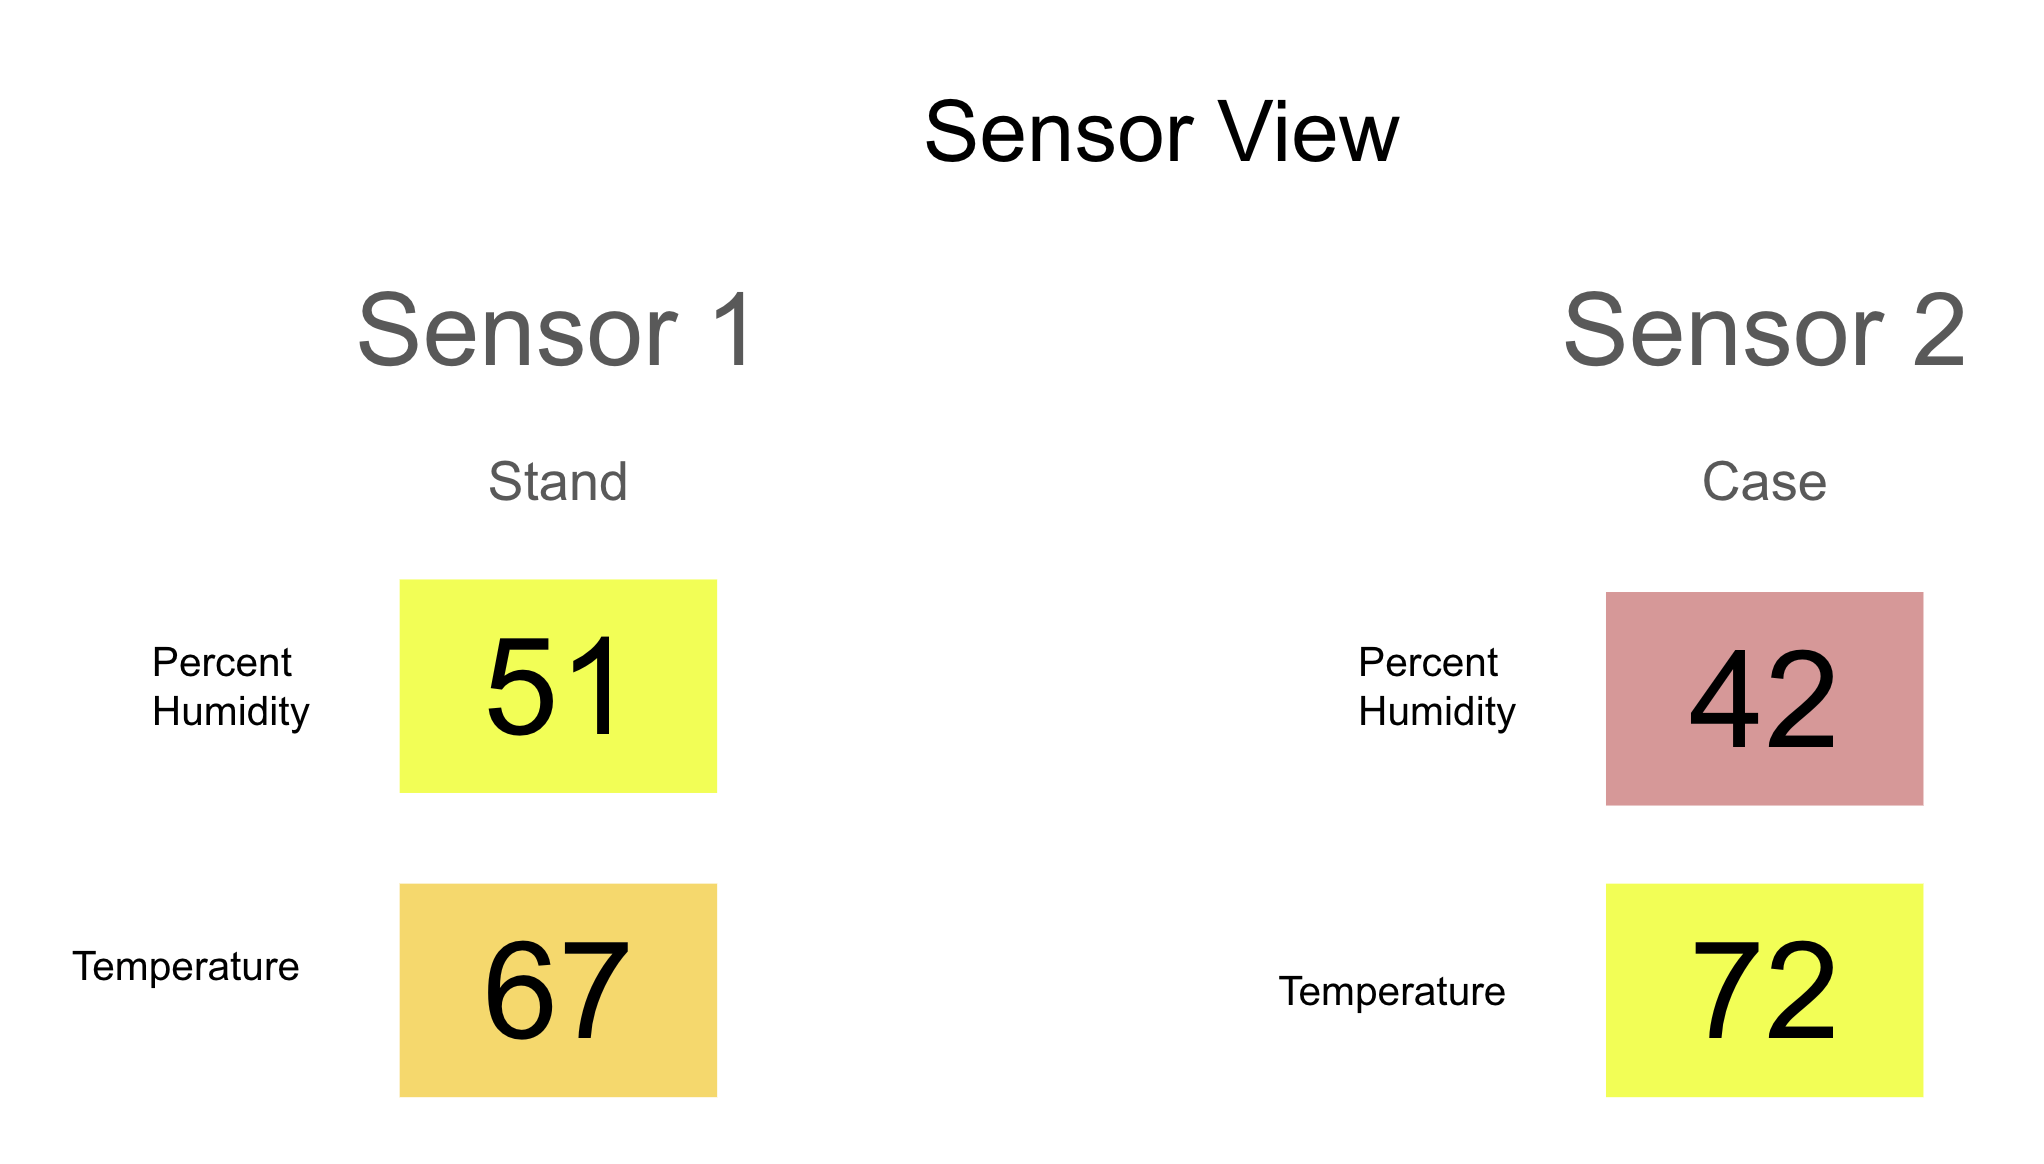
\includegraphics[width=\textwidth]{images/sensor-overview.png}
      \end{column}
      \begin{column}{.5\textwidth}
        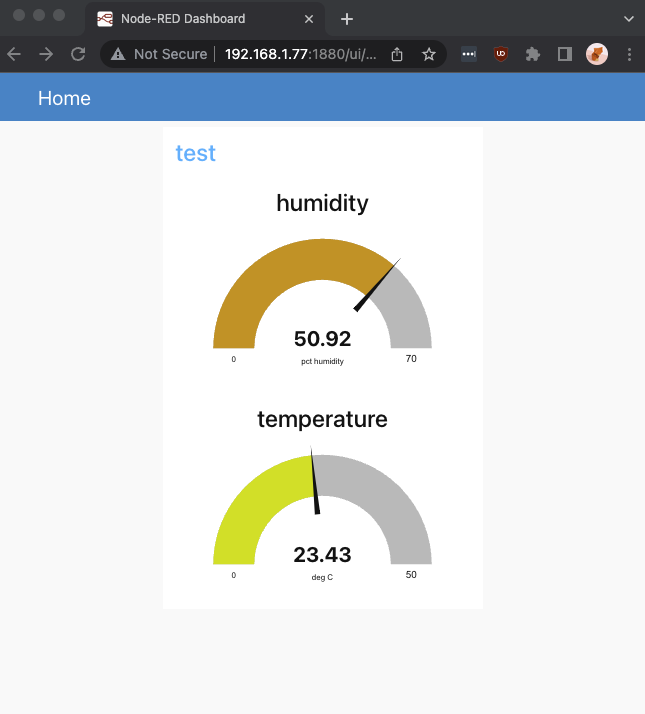
\includegraphics[width=\textwidth]{images/test-dashboard.png}
      \end{column}
    \end{columns}
  \end{frame}
  \begin{frame}{\sectitle}
    \begin{itemize}
      \item Sensor/server relationship $\rightarrow$ sensors now publish on a fixed schedule, while the server just listens (via Mosquitto MQTT)
      \item Handling sensor ``wonkiness'' $\rightarrow$ take 20 super-fast averaged readings every 30 seconds to moderate weird readings
      \item More heavily websocket-based (JavaScript \& socket.io) rather than db-based
    \end{itemize}
  \end{frame}


  \renewcommand{\sectitle}{Timeline}
  \begin{frame}{\sectitle}{Burn-Up: Estimated vs Actual}
    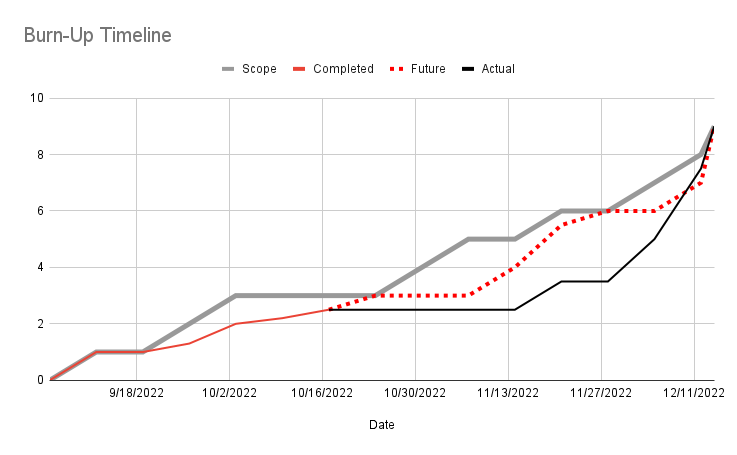
\includegraphics[width=\textwidth]{images/burn-up.png}
  \end{frame}
  \begin{frame}{\sectitle}{Retrospective}
    \begin{columns}
      \begin{column}{.5\textwidth}
        \textbf{Did we meet timeline goals?}\\\textit{yes and no\dots}\\
        \vspace*{1em}
        ``Confounding factors'':
        \begin{itemize}
          \item Changing core system $\rightarrow$ from "Pi controls all" to "sensors control themselves"
          \item General sensor / embedded coding (C++)
          \item Websockets / socket.io
        \end{itemize}
      \end{column}
      \begin{column}{.5\textwidth}
        \centering
\includegraphics[scale=.25]{images/IMG_7529.png}
      \end{column}
    \end{columns}
  \end{frame}
  % \begin{frame}{\sectitle}{Key Points}
  %   \begin{itemize}
  %     \item Early October -- End of October: sensor prototyping and finalize code for sensor ($\approx 1-2$ more weeks)
  %     \item Early November: Build backend and analysis capabilities ($\approx 1-2$ weeks)
  %     \item Late November: Build frontend -- user interface ($\approx 2-3$ weeks)
  %     \item Early December: Bring everything together + final touches ($\approx 1$ week)
  %   \end{itemize}
  % \end{frame}


  \renewcommand{\sectitle}{Action Shots}
  \section{\sectitle}
  \begin{frame}{\sectitle}
    \begin{columns}
      \begin{column}{.5\textwidth}
        \centering\includegraphics[width=\textwidth]{images/IMG_7538.png}
      \end{column}
      \begin{column}{.5\textwidth}
        \centering\includegraphics[width=\textwidth]{images/IMG_7539.png}
      \end{column}
    \end{columns}
  \end{frame}


  \begin{frame}{Bonus}{\texttt{technology}}
    \centering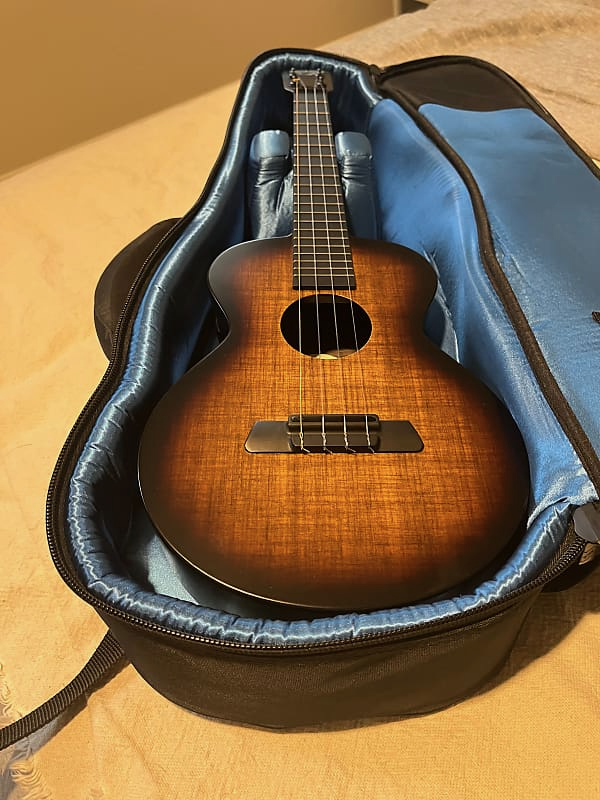
\includegraphics[scale=.3, angle=270]{images/IMG_5145.png}
  \end{frame}


  \renewcommand{\sectitle}{What's Next?}
  \section{\sectitle}
  \begin{frame}{\sectitle}
    \begin{itemize}
      \item Battery power $\rightarrow$ investigate sleep/wake \& power draw
      \item Increased database connectivity $\rightarrow$ trends \& logging capabilities
      \item DNS $\rightarrow$ have a custom URL rather than something like \texttt{192.168.1.83:8080}
      \item Security $\rightarrow$ currently nothing securing Mosquitto \& allows anonymous publishing
      \item Soft Access Point $\rightarrow$ allow users to change sensor settings after flashing
    \end{itemize}
  \end{frame}


  \renewcommand{\sectitle}{Demo Screenshots}
  \section{\sectitle}
  \begin{frame}{\sectitle}
    \begin{center}
      \huge Just in case anything blows up\dots
    \end{center}
  \end{frame}
  \begin{frame}{\sectitle}{Empty Home Screen}
    \centering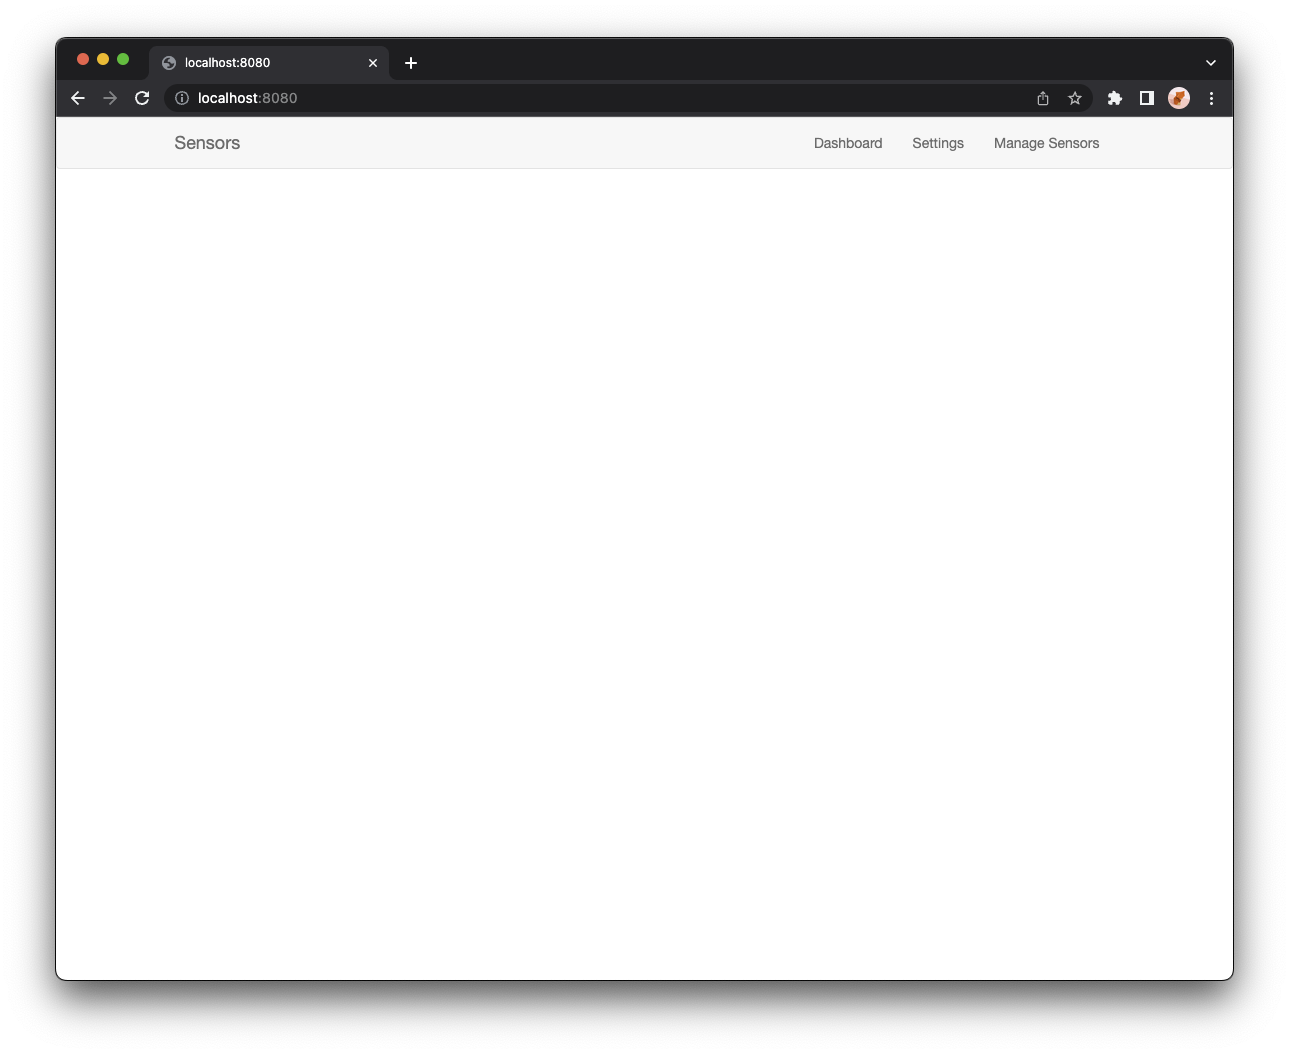
\includegraphics[width=.75\textwidth]{images/01-home.png}
  \end{frame}
  \begin{frame}{\sectitle}{Adding a Sensor}
    \centering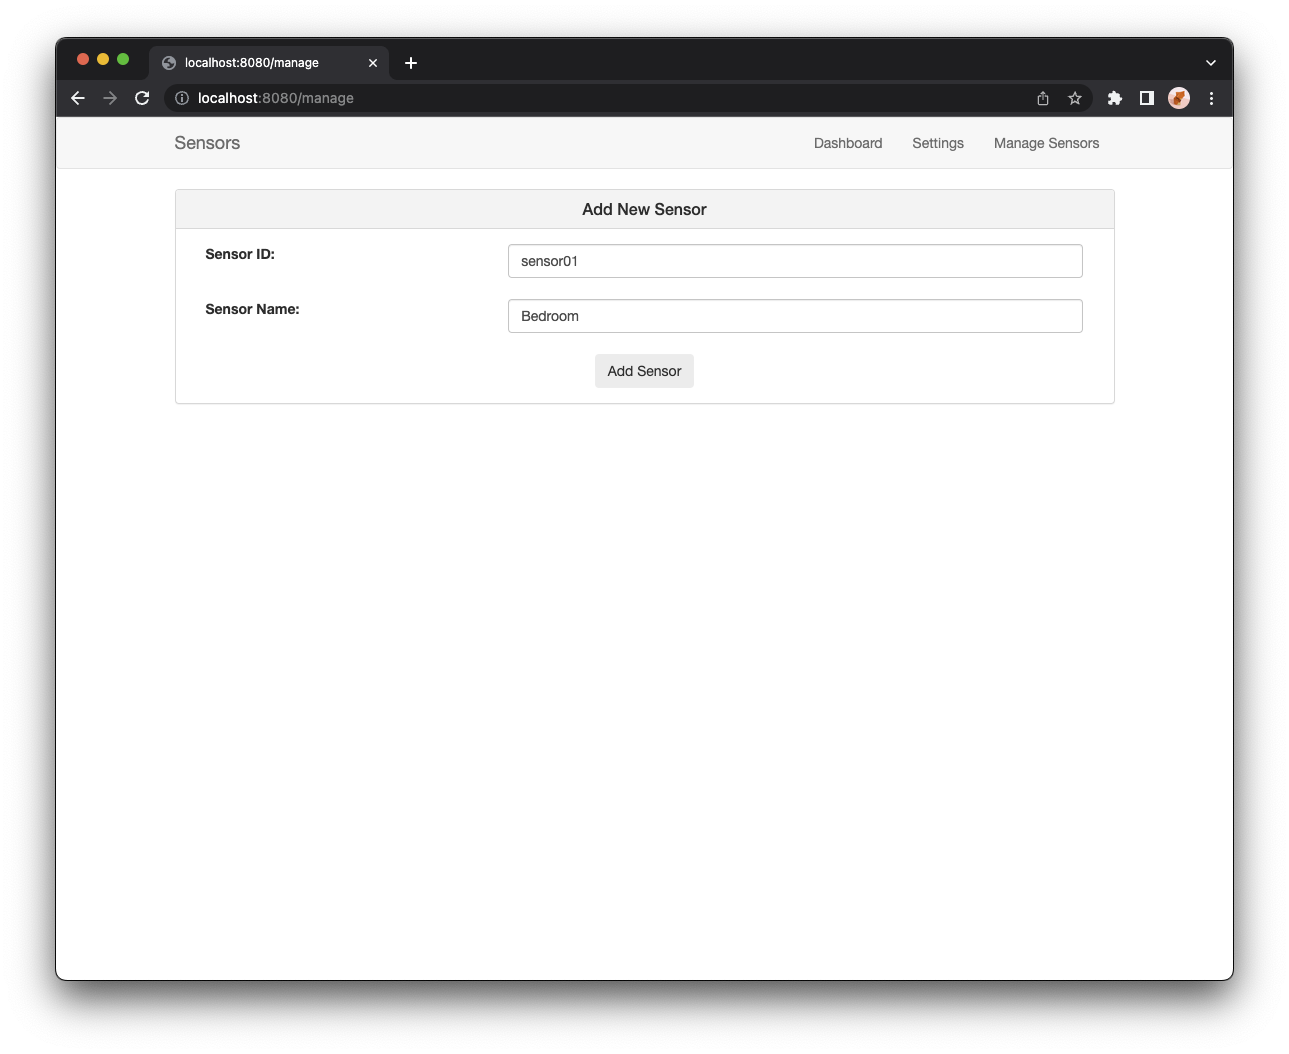
\includegraphics[width=.75\textwidth]{images/02-add.png}
  \end{frame}
  \begin{frame}{\sectitle}{Populated Home Screen}
    \centering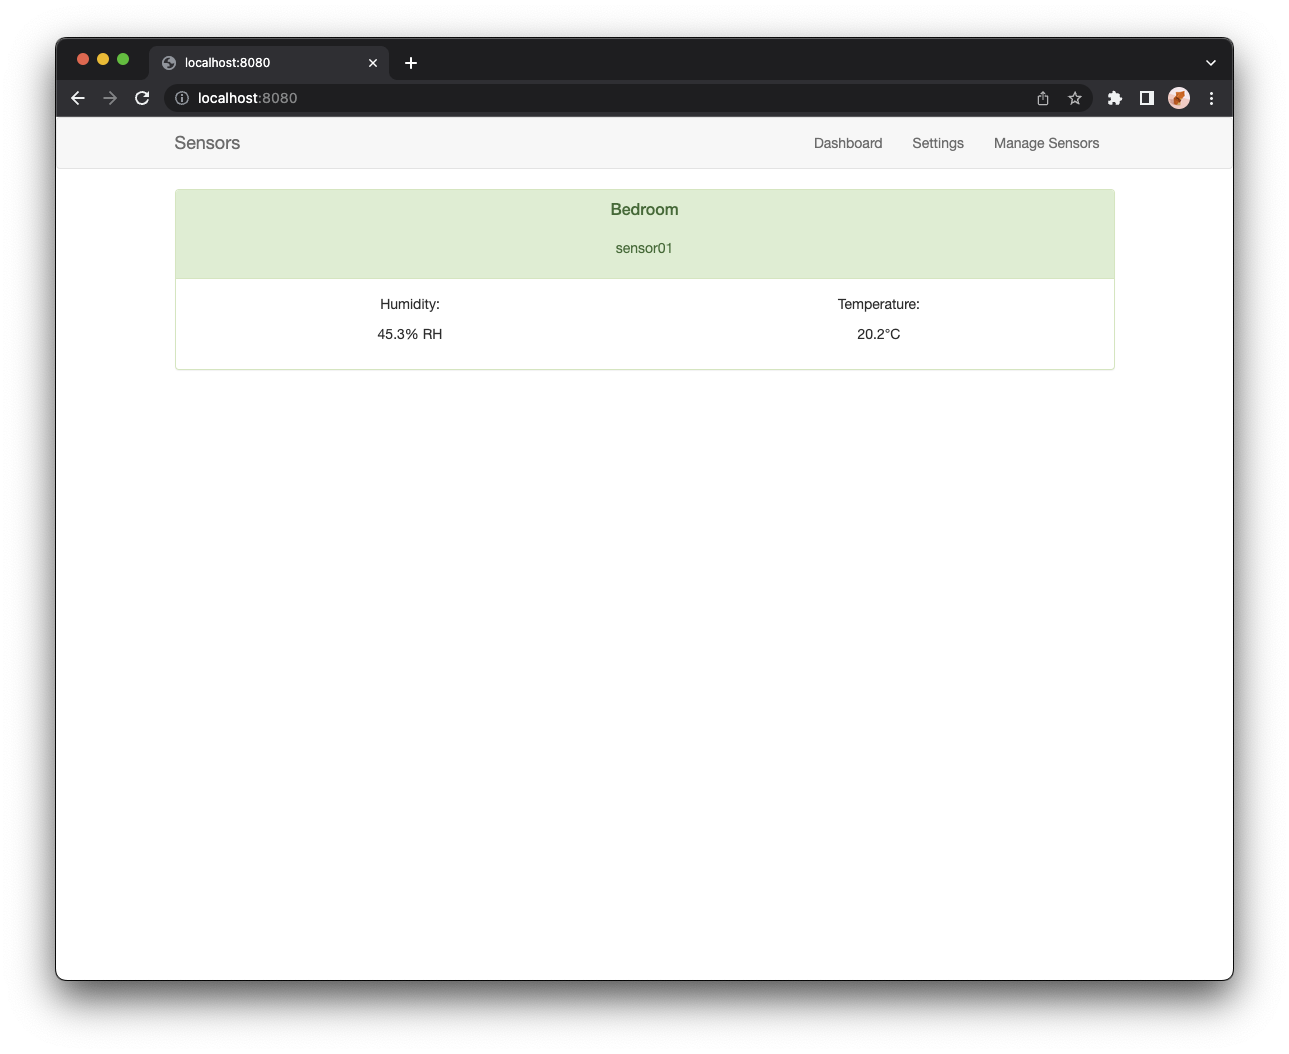
\includegraphics[width=.75\textwidth]{images/03-added.png}
  \end{frame}
  \begin{frame}{\sectitle}{Out-of-Range Alert}
    \centering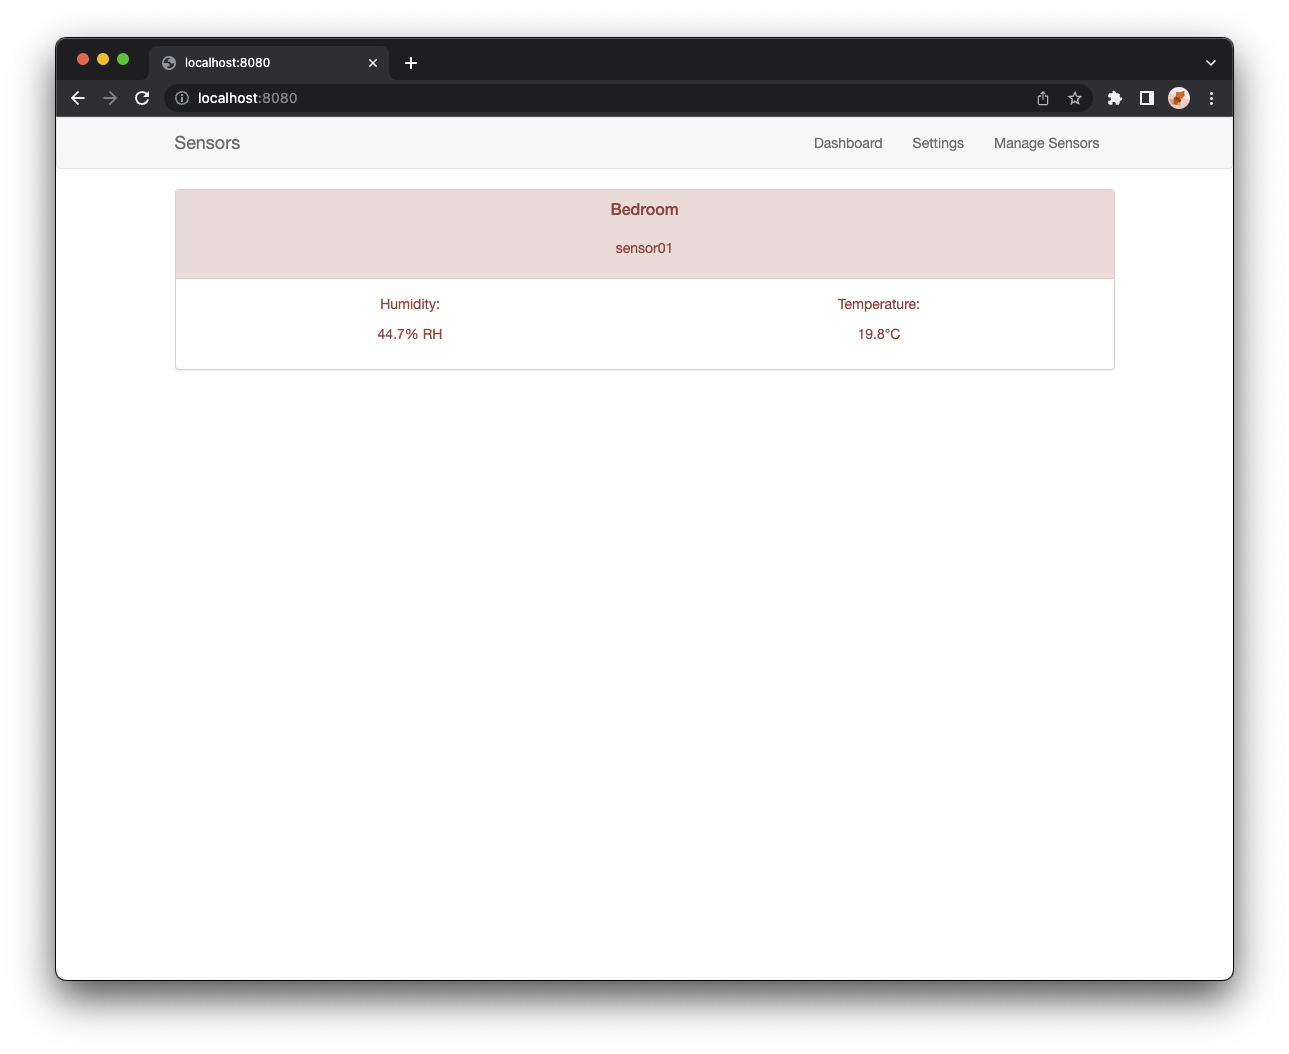
\includegraphics[width=.75\textwidth]{images/04-out_of_range.png}
  \end{frame}
  \begin{frame}{\sectitle}{Settings Menu}
    \centering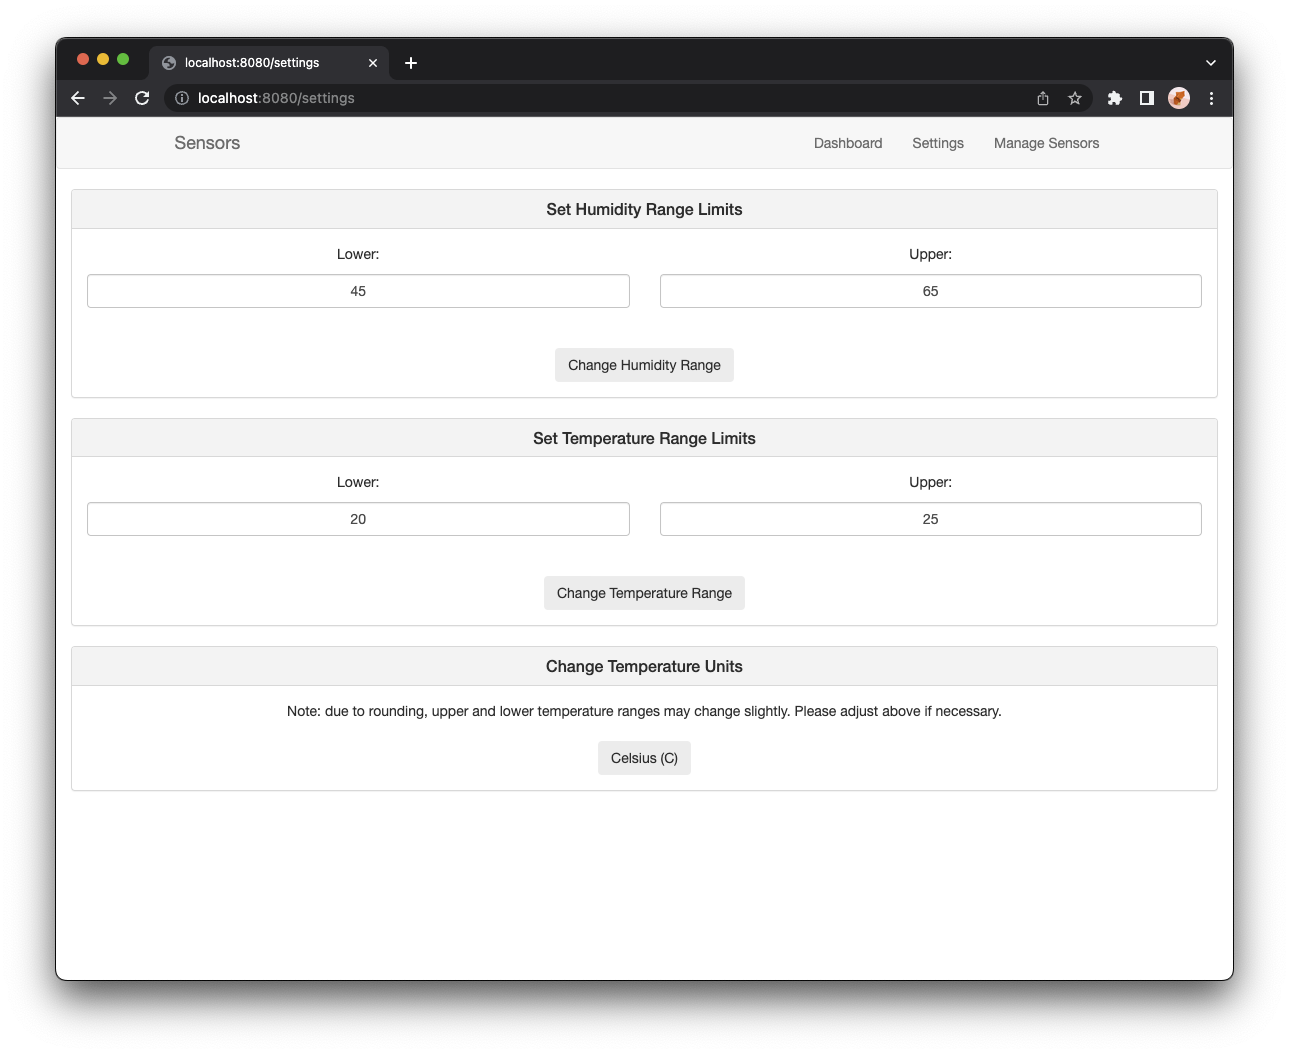
\includegraphics[width=.75\textwidth]{images/05-settings.png}
  \end{frame}
  \begin{frame}{\sectitle}{Dashboard in Fahrenheit}
    \centering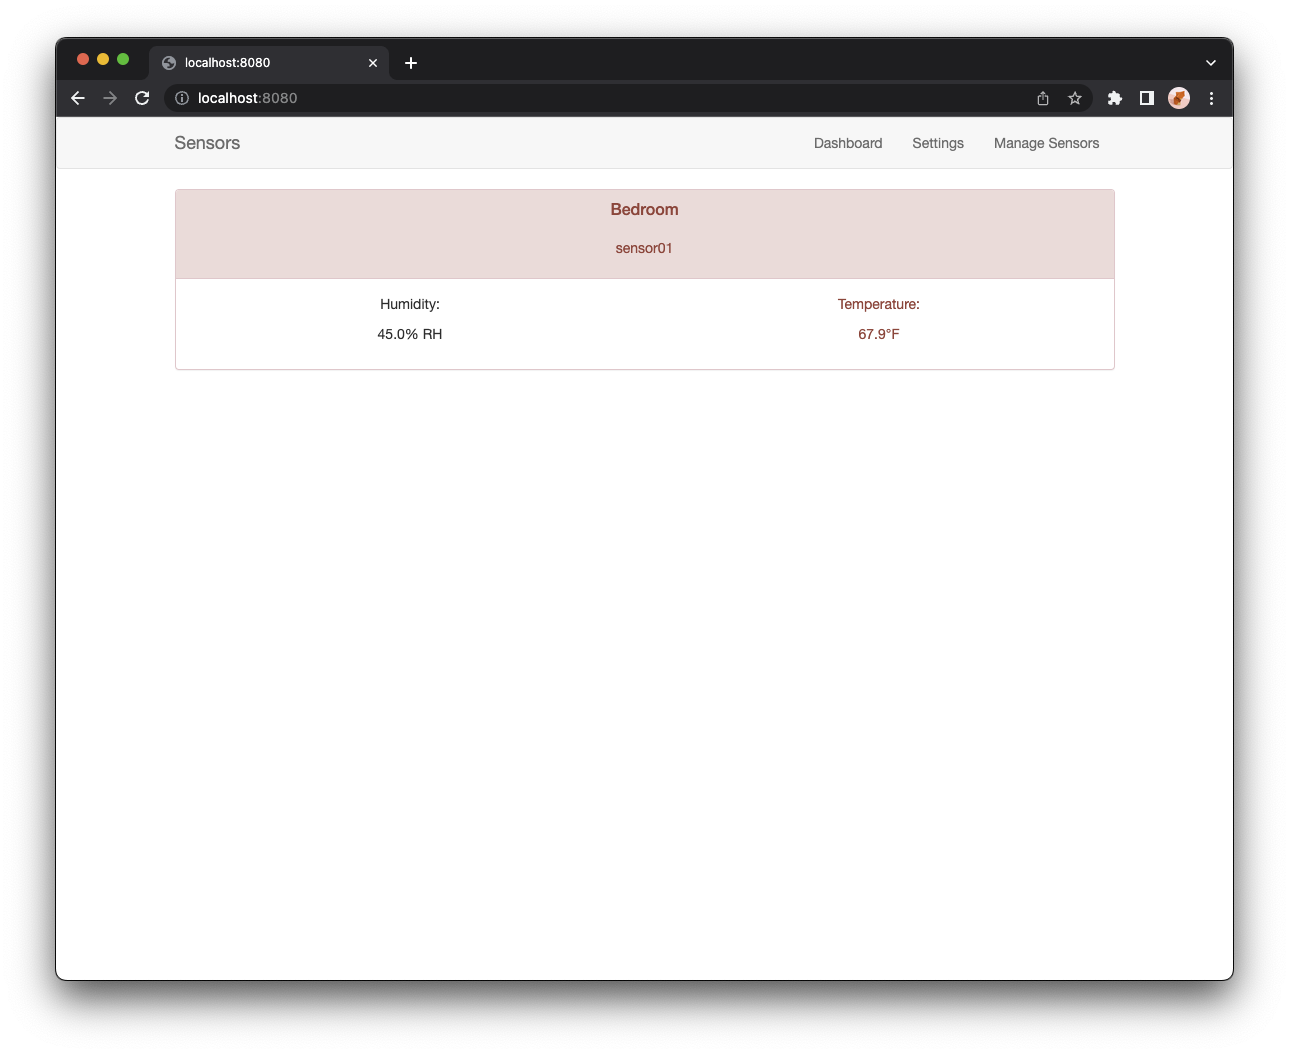
\includegraphics[width=.75\textwidth]{images/06-in_F.png}
  \end{frame}
  \begin{frame}{\sectitle}{Removing a Sensor}
    \centering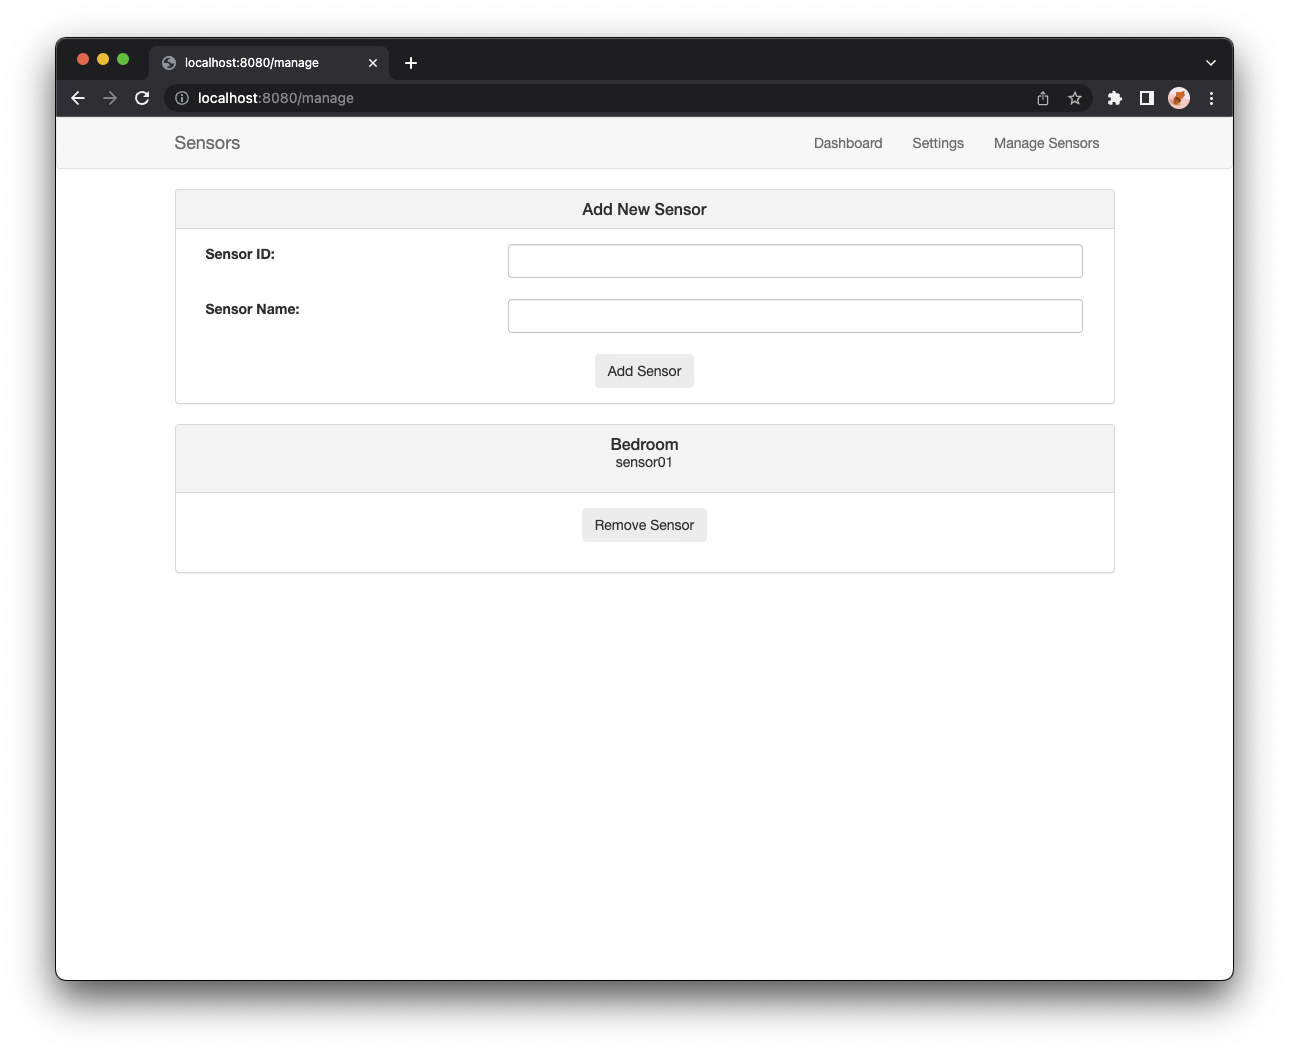
\includegraphics[width=.75\textwidth]{images/07-remove.png}
  \end{frame}
  \begin{frame}{\sectitle}{Multiple Sensors}
    \centering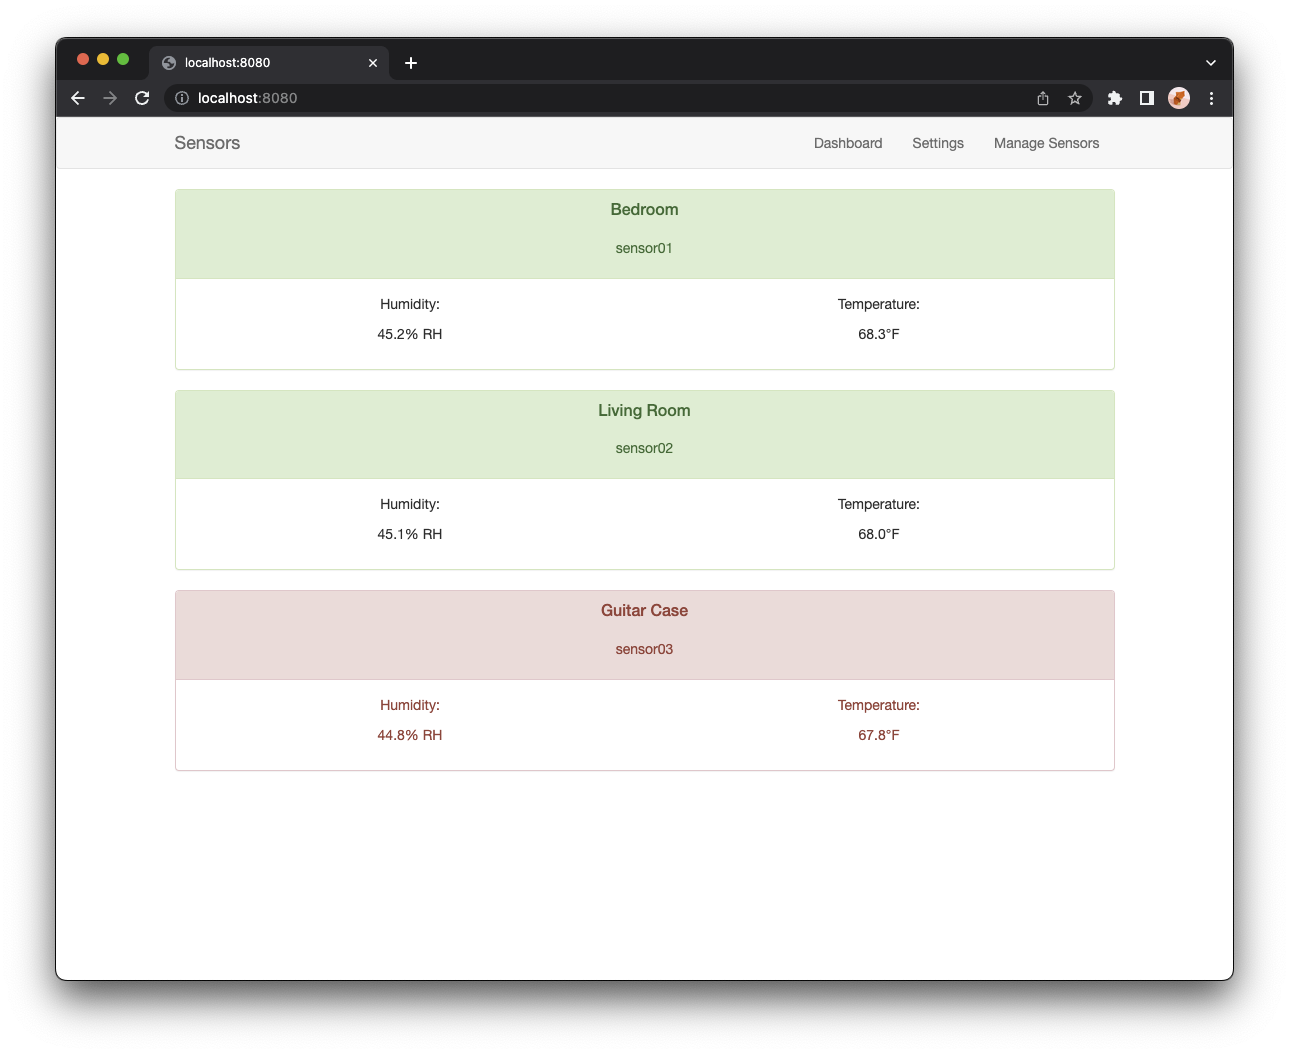
\includegraphics[width=.75\textwidth]{images/08-many.png}
  \end{frame}



\end{document}